%
%  untitled
%
%  Created by Travis Johnson on 2013-06-17.
%  Copyright (c) 2013 . All rights reserved.
%
\documentclass[twocolumn,openany]{book}

% Use utf-8 encoding for foreign characters
\usepackage[utf8]{inputenc}

% Setup for fullpage use
\usepackage{savetrees}

% Uncomment some of the following if you use the features
%
% Running Headers and footers
%\usepackage{fancyhdr}

% Multipart figures
%\usepackage{subfigure}

% More symbols
\usepackage{amsmath} 
\usepackage{amssymb}
\usepackage{latexsym}

% Surround parts of graphics with box
\usepackage{boxedminipage}

% Package for including code in the document
\usepackage{listings}

% If you want to generate a toc for each chapter (use with book)
\usepackage{minitoc}

% This is now the recommended way for checking for PDFLaTeX:
\usepackage{ifpdf}

%\newif\ifpdf
%\ifx\pdfoutput\undefined
%\pdffalse % we are not running PDFLaTeX
%\else
%\pdfoutput=1 % we are running PDFLaTeX
%\pdftrue
%\fi

\ifpdf
\usepackage[pdftex]{graphicx}
\else
\usepackage{graphicx}
\fi
\title{Princeton \\ RTG Summer School \\in Financial Mathematics (2013)}
\author{ Travis Craig Johnson \thanks{Dept.~of Eng.~Sci.~and App.~Math., Northwestern University, Evanston, IL 60208, USA. email: \texttt{traviscj@traviscj.com}}}

\date{2013-06-17}

\begin{document}

\ifpdf
\DeclareGraphicsExtensions{.pdf, .jpg, .tif}
\else
\DeclareGraphicsExtensions{.eps, .jpg}
\fi

\maketitle

\chapter{Administrivia}
\section{Lecturers}
\begin{enumerate}
	\item Rene Carmona (Princeton University)
	\item Rama Cont (Imperial College London)
	\item Michael Coulon (Princeton University)
	\item Jean-Pierre Fouque (UC Santa Barbara)
	\item Johannes Muhle-Karbe (ETH Zurich)
	\item Alexander Schied (University of Mannheim)
	\item Ronnie Sircar (Princeton University)
	\item Glen Swindle (Scoville Risk Partners LLC \& NYU)
\end{enumerate}
\section{Times}
\begin{enumerate}
	\item 9-9:50 - Lecture
	\item 10-10:50 - Lecture
	\item 11-11:30 - Break
	\item 11:30-12:20 - Lecture
	\item 12:30-14:00 - Lunch
	\item ?? 13:30-14:00 - Special Q\&A Session ??
	\item 14:00-14:50 - Lecture
	\item 15:00-15:50 - Guest Lecture
\end{enumerate}

\section{Locations}
\begin{enumerate}
	\item Week 1: Friend Center room 006
	\item Week 2: Computer Science Building room 104
\end{enumerate}

\section{Links}
\begin{enumerate}
	\item https://orfe.princeton.edu/rtg/fmsummer/reading
	\item https://github.com/traviscj/fmsummer
\end{enumerate}

\part{Systemic Risk}
% June 17
\chapter{Systemic Risk 1 - Fouque}
\section{History}
\begin{enumerate}
	\item 60's and 70's: 
	\begin{enumerate}
		\item Problem of Portfolio Allocation (Mean-Variance/Markovitz/)
		\item Option Pricing(1973) (Black-Scholes/etc)
	\end{enumerate}
	\item 90's:
	\begin{enumerate}
		\item Local Volatility
		\item Stochastic Volatility
	\end{enumerate}
	\item 2000's:
	\begin{enumerate}
		\item Credit - Taking into account the possibility of default(of company, counterparty, etc)
		\item Credit Basket - structuring risk(Mortgages)
		\item Credit Default Swap
		\item Collatorized Default Options - Huge Huge Market.
		\item Financial Crisis - Mortgages were completely mispriced.
	\end{enumerate}
	
	\item 2008-2010:
	\begin{enumerate}
		\item NIF: National Institute of Finance (for doing research on the banking \emph{system})
		\item Handbook on Systemic Risk: Cambridge
		\item Dodd-Frank: Created Office of Financial Research (under the treasury department)
	\end{enumerate}
\end{enumerate}

% \begin{definition}\label{def:systemic_risk}
% 	We define \emph{systemic risk}: 
% 	\begin{enumerate}
% 		\item a lot of defaults
% 		\item lack of liquidity
% 	\end{enumerate}
% \end{definition}

\section{Systemic Risk}
Can consider from many views: mathematics, statistics, etc.

Two main approaches:
\begin{enumerate}
	\item Coupled Diffusions: Continuous time
	\item Networks
\end{enumerate}

The starting point is Brownian Motion. Suppose we start with an asset:
\begin{equation}
	dS_t = \mu S_t dt
\end{equation}
which we can solve by
\begin{equation}
	S_t = S_0e^{\mu t}
\end{equation}
Okay, but usually we don't know the $\mu$, and there is some noise! How can we add noise? Since $\mu$ is the return, maybe by adding some \emph{white noise}
\begin{equation}
	dS_t = S_t(\mu dt + \text{Noise})
\end{equation}
where the Noise term is given by Brownian Motion, which has the form
\begin{equation}
	\sigma dW_t
\end{equation}
with $\sigma > 0$, and $(W_t)_{t\geq 0}$ for $t\leq T$. The properties of Brownian Motion:
\begin{enumerate}
	\item $W_0=0$
	\item $W_t$ is continuous
	\item Independent, increments
	\item If we consider
	\begin{equation}
		0 < t_1 < ... < t_n \leq T
	\end{equation}
	then it gives rise to many differences:
	\begin{equation}
		(W_{t_1} - W_{t_0}, W_{t_2} - W_{t_1}, ... W_{t_n} - W_{t_{n-1}})
	\end{equation}
	such that
	\begin{equation}
		\mathcal{D}(w_t - w_s) = \mathcal{N}(0, t-s)
	\end{equation}
\end{enumerate}
A bit of Brownian Motion History:
\begin{enumerate}
	\item Brown
	\item Buchelier (1900)
	\item Albert Einstein (1905): Heat Equation/Brownian Motion tie-in
	\item Weiner (1930s): Constructed Brownian Motion: Construct a measure over all continuous trajectories
	\item Ito (1940s): Figures out chain rule for brownian motion
	\item Samuelson (1960s): Generalized Brownian Motion
\end{enumerate}

If we have a bounded function $f(t)$ where
\begin{equation}
	\sum_{0}^T \left( f(t_{i+1}) - f(t_i) \right) < \infty
\end{equation}
If we have a brownian motion instead,
\begin{equation}
	\sum_0^T \left| W_{t_{i+1}} - W_{t_i} \right| \to \infty
\end{equation}

Book Reference: Carson \& Tree???

\section{Hitting Times}
Draw a plot:
\begin{enumerate}
	\item time on horizontal axis
	\item y = brownian motion on vertical axis
	\item line $y=\alpha$.
\end{enumerate}

\begin{figure}[htbp]
	\centering
		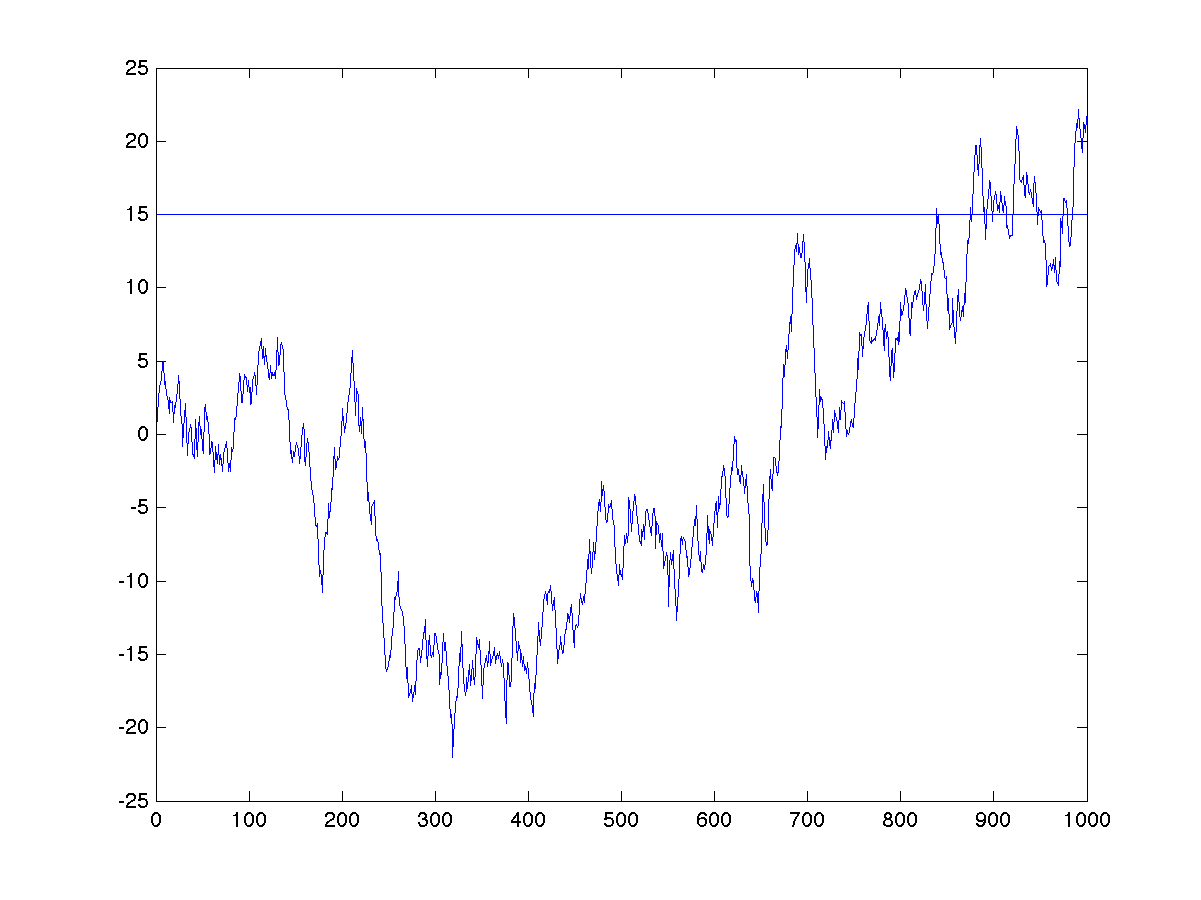
\includegraphics[width=.9\linewidth]{brownian_motion.png}
	\caption{caption}
	\label{fig:label}
\end{figure}

We are interested in the time $\tau_{\alpha}$, defined by
\begin{equation}
	\tau_a = \inf \{ t>0 : W_t \geq a \}
\end{equation}
(We are really looking for $W_t=a$)

We can instead think
\begin{equation}
	\{ \tau_a\leq t \} = \{ \max_{0\leq s \leq t} W_s \geq a \}
\end{equation}
Then
\begin{equation}
	\tilde{W}_t = W_t \Theta_{t \leq \tau} + (2a - W_t) \Theta_{t > \tau}
\end{equation}
is a Brownian Motion. RP.

Now suppose we want to find the probability:
\begin{align}
	\mathbb{P}(\tau& \leq t, |W_t-a|> b) \\
	=& \mathbb{P}(\tau \leq t, W_t > a+b) + \mathbb{P}(\tau \leq t, W_t < a-b)\\
	=& 2\mathbb{P}(\tau \leq t, W_t > a+b)\\
	=& 2N_{(0,t)}(-a-b)
\end{align}
But we also know that
\begin{equation}
	\mathbb{P}(\tau \leq t) = 2N_{(0,t)}(-a)
\end{equation}

A few remarks:
\begin{enumerate}
	\item $\tau$ is predictable. We say that $\tau$ is \emph{announced} by a sequence $\tau_n$, the hitting time of $a-\frac1n$.
	\item Large Deviations: Consider the probability of a very large deviation ($a \to \infty$)
	\begin{equation}
		\mathbb{P}(\tau_a \leq t) \sim e^{-\frac{a^2}{2t}}
	\end{equation}
	where we mean this in term of the log.
\end{enumerate}


\chapter{Systemic Risk 2 - Fouque}
\section{Joint Distributions}
Consider the joint distribution of $(\tau,W_t)$. We can think of this as
\begin{equation}
	``\mathbb{P}(\tau\leq t, W_t = v)'' = \begin{cases}
		\mathbb{P}(W_t = v) & \text{if } v > a\\
		\mathbb{P}(W_t=2a-v) & \text{if } v < a
	\end{cases} = \begin{cases}
		g(v)\\
		g(2a-v)
	\end{cases}
\end{equation}

For nonstandard Brownian Motions,
\begin{equation}
	X_t = x + \mu t + \sigma W_t
\end{equation}
And then
\begin{equation}
	\tau = \inf \{ t> 0, x_t \geq a \}
\end{equation}
So then,
\begin{align}
	x_t \geq a  \iff& (x+\mu t + \sigma W_t \geq a)\\
	\iff& \mu t + \sigma W_t \geq a-x\\
	\iff& \frac{\mu}{\sigma} t + w_t \geq \frac{a-x}{\sigma}
\end{align}
Define $\theta=\frac{\mu}{\sigma}$, and $\tilde{a}=\frac{a-x}{\sigma}$.

Then we have that
\begin{equation}
	W_t + \theta t \equiv W_t^\theta
\end{equation}
Then Girsanov's Thm is 
\begin{equation}
	M_t^\theta = e^{-\theta W_t - \frac{1}{2}\theta^2t}
\end{equation}
Then
\begin{equation}
	\mathbb{E}(M_t^\theta) = 1
\end{equation}
and
\begin{equation}
	\frac{dP^\theta}{dP}|_{f_x} = M^\theta_t
\end{equation}

We can show that $W_t + \theta t \equiv W_t^\theta$ is a brownian motion under $\mathbb{P}^\theta$. So next,
\begin{equation}
	\mathbb{E}^\theta \left( x / F_s\right) = \frac{1}{M^\theta_s} \mathbb{E}(X M^\theta_t / F_s) 
\end{equation}
Then we will be able to show
\begin{equation}
	\mathbb{E}^\theta \left( e^{iu(W_t^\theta - W_s^\theta)} \right) = e^{-\frac{\mu^2}{2}(t-s)}
\end{equation}
Why do we care about all of that? Well, we can do the following:
\begin{equation}
	\tau = \inf \{ t> 0, W_t^\theta \geq \tilde{a} \}
\end{equation}
Then
\begin{equation}
	\mathbb{P}(\tau \leq t) = \mathbb{E}(\Theta_{\tau \leq t}) = \mathbb{E}^\theta \equiv \left( \Theta_{\tau \leq t} \frac{d\mathbb{P}}{d\mathbb{P}^\theta} \right)
\end{equation}
We can use the joint distribution of $(\tau, W_t^\theta)$.
\begin{equation}
	= N( -\frac{a - x - \mu t}{\sigma \sqrt{t}}) + e^{\frac{2(a-x)\mu)}{\sigma^2}} N(-\left( \frac{a - x + \mu t}{\sigma \sqrt{t}}\right))
\end{equation}

\section{Geometric Brownian Motion}
Now consider
\begin{equation}
	dS_t = S_t (\mu dt + \sigma dW_t)
\end{equation}
which is a stochastic differential equation. We should think of this as a convient notation for something more complicated. Basically,
\begin{equation}
	S_t dW_t \to \int_0^t S_a dW_a
\end{equation}

We will use Ito's lemma which lets us do the chain rule with a brownian motion:
\begin{equation}
	dg(W_t) = g'(W_t) dW_t + \frac12 g''(W_t)dt
\end{equation}
where $g(t,W_t)$ is once differentiable in $t$ and twice differentiable in $W_t$. Then if we have
\begin{equation}
	dX_t = \varphi_t dt + \psi_t dW_t
\end{equation}
then
\begin{equation}
	dg(X_t)  = g'(X_t)dX_t + \frac{1}{2} g''(X_t)d\langle x\rangle_t
\end{equation}
Then an SDE like
\begin{equation}
	dX_t = b(t,X_t)dt + \sigma(t,X_t) dW_t
\end{equation}
has a solution like
\begin{equation}
	S_t = S_0 e^{(\mu - \frac{\sigma^2}{2})t} + \sigma W_t
\end{equation}

\section{Passage Time}
Now consider
\begin{equation}
	dS_t = S_t(\mu dt + \sigma dW_t) = S_t(r dt + \sigma(dW_t + \frac{\mu-r}{\sigma}dt))
\end{equation}
well then, $\mathbb{P}^*$: $e^{-rt}S_t$ is a martingale.

\section{Defaultable Bond}
Now we want to have a defaultable bond. The bond starts at $S_0$ and has a default value of $D$(if it touches $D$ before maturity time $T$ then we have no payout, otherwise get 1.) So then the price of the bond is
\begin{equation}
	\mathbb{P}^D_{(0,T)} = \mathbb{E}^*(\Theta_{\tau > T}) = \mathbb{P}^*(\tau > T).
\end{equation}
So now we consider
\begin{equation}
	\{ \inf_{0 < t \leq T} S_0 e^{(r- \frac{\sigma^2}{2})t + \sigma W_t} > 0 \} 
\end{equation}
By taking the logarithm, we get a nonstandard brownian motion, which we can evaluate. By some computation, we can get
\begin{equation}
	\mathbb{P}^\theta(0,T) = e^{-rT}\left[ N(d_2^+) - \left(\frac{S_0}{D} \right)^{1-\frac{2r}{\sigma^2}}N(d_2^-) \right]
\end{equation}
with
\begin{equation}
	d_2^{\pm} = \frac{\pm \log \frac{S_0}{D} + \left(r - \frac{\sigma^2}{2} \right)t}{\sigma \sqrt{t}}
\end{equation}

The main ingredients here were reflection principle and change of measure. Alternatively, one could do this completely with partial differential equations.

\section{Yield}
We can represent the yield by
\begin{equation}
	y(0,t) = -\frac{1}{T}\log \frac{\mathbb{P}^D(0,T)}{\mathbb{P}(0,T)}
\end{equation}

\subsection{Example}
Consider some bond $B_1$ with a 10\% default rate. This is too risky for index funds, and not risky enough for hedge fund.

A financial engineer will do this: Buy two bonds, $B_1$ and $B_2$ (both with 10\% default rate), then stack them. Now
\begin{enumerate}
	\item pays if 2 defaults: 0.99
	\item pays if 1 default: .8
\end{enumerate}
What's the problem? We assumed independence.

In credit, the main risk was correlation of default. This is not really computable.

Consider two processes $W_t^{(1)}$, $W_t^{(2)}$ and the hitting times $\tau^{(1)}$ and $\tau^{(2)}$ try and figure the probability $\mathbb{P}(z^{(1)} > T; z^{(2)}> T)$, well, it's hard to quantify. If 

\section{Systemic Risk}
Usually we will consider the log-capitalization of Banks, and in particular multiple banks:
\begin{equation}
	dX_t^i = \mu_t^i dt + \sigma^i dW_t^i.
\end{equation}
\subsection{Toy Model}
We can consider the drift of capitalization, which includes some coupling of the systems.
\begin{equation}
	dX^i_t = \frac{a}{N} \sum_{j\ne i} (X^j_t - X_t^i)dt + \sigma^i (\rho dW_t^\theta + \sqrt{1-\rho^2} dW_t^i)
\end{equation}
where the $W^i_t$ are independent.
What is the intuition here? That borrowing and lending goes on between the banks. This is related to flocking and swarming models.

What other mathematical model behaves this way(where we have randomness but also attraction)? ornstein uhlenbeck process:
\begin{equation}
	dY_t = a(m-y_t)dt + \sigma dW_t,
\end{equation}
which we know how to solve:
\begin{equation}
	Y_t = m + (y-m)e^{-at} + \sigma e^{-at} \int_0^t e^{as}dW_p
\end{equation}
And we know that this is $\mathcal{N}(m, \frac{\sigma^2}{2a})$.

Next step is:
\begin{equation}
	d(\frac{1}{N} \sum_{i=1}^N X_t^i ) = 0 dt + \sigma \rho dW_t^0 + \frac{\sigma\sqrt{1-\rho^2}}{N} \sum_{i=1}^N dW_t^i.
\end{equation}
Now consider if $X_0^i=x_0^i=0$, which gives
\begin{equation}
	\bar{x}_t = \frac{1}{N}\sum_{i=1}^N X_t^i = \sigma \rho W_t^0 + \frac{\sigma \sqrt{1-\rho^2}}{N} \sum_{i=1}^N W_t^i
\end{equation}
If we take $\rho=0$ for a second, then
\begin{equation}
	\bar{x}_T \sim \frac{\sigma}{\sqrt{N}}\tilde{W}_t
\end{equation}


\chapter{Systemic Risk Day 3}
We will continue considering the equation governing the log-capitalization of the banks
\begin{equation}
	dX_t^i = \frac{a}{N} \sum_{j=1}^N (x_t^j - x_t^i)dt + \sigma (\rho dW_t^0 + \sqrt{1-\rho^2} dW_t^i)
\end{equation}
where $W^0$, ..., $W^N$ are independent brownian motions and $a$ represents the speed of trading. We can further consider the mean over all these,
\begin{equation}
	\bar{X}_t = \frac{1}{N} \sum_{i=1}^N X_t^i
\end{equation}
which lets us write as
\begin{equation}
	d X_t^i = a (\bar{X}_t - X_t^i)dt + \text{Noise}
\end{equation}
where the mean is governed by
\begin{equation}
	d\bar{X}_t = \sigma\rho dW_t^0 + \frac{\sigma \sqrt{1-\rho^2}}{N}\sum_{i=1}^N dW_t^i
\end{equation}
Which is equivalent to [ed: is this true?]
\begin{equation}
	= \sigma \sqrt{\rho^2 - \frac{1-\rho^2}{N}}dB_t
\end{equation}
This gives rise to a flocking behavior--all the banks will follow the mean--at least as long as the mean is large.

Consider the case where $\rho=0$ which gives
\begin{equation}
	\frac{\sigma}{\sqrt{N}}dB_t.
\end{equation}
We will count a bank as defaulting when it hits some default amount $D<0$. We can consider the event
\begin{equation}
	\left\{ \min_{0\leq t \leq T} \bar{X}_t < D \right\}
\end{equation}
And in particular, we can calculate the probability of default,
\begin{equation}
	\mathbb{P}(\min_{0\leq t \leq T} \bar{X}_t < D) 
	= \mathbb{P}(\tau \leq t) 
	= 2\mathcal{N}(\frac{D\sqrt{N}}{\sigma\sqrt{T}})
	\sim e^{-\frac{D^2 N}{\sigma^2 T}}
\end{equation}

Another interesting regime: $\rho=0$. Then
\begin{equation}
	\bar{X}_t \sim \sigma \rho W_t^0
\end{equation}
and
\begin{equation}
	\mathbb{P}(\bar{\tau} \leq t) = 2 \mathcal{N}(\frac{D}{\sigma \rho \sqrt{T}})
\end{equation}
But this actually isn't too interesting.

Another one: $N\to \infty$ with $\rho=0$. We must be very careful here--taking $N\to\infty$ completely misses the systemic risk. That is because $\bar{X_t}\to 0$. But we could consider $N\to\infty$ but then reconsider with $N$ large but finite later. In this case, the $(X_t^i)$ become OUs, which are independent.  Then
\begin{equation}
	d X_t^i = -a X_t^i + \sigma dW_t^i
\end{equation}
and we need to find the hitting time of an OU(which is annoying, but possible).


\section{Other models}
\subsection{Garnier - Papanicolaou - Wang}
Here, we replace the hitting times with a double well potential.

That is, we create a double-well potential: $V(x) = a x^4 + b x^2$ (with $a>0$, $b<0$). Then the equation becomes
\begin{equation}
	dX_t^i = h V'(X_t^i) dt + a \sum_{j=1}^N (X_t^i - X_t^j) dt + \sigma dW^i_t
\end{equation}


\section{Games}
Work done with Carmona and Sun. We want the bank to be able to do something. To start, consider
\begin{equation}
	dX_t^i = \frac{a}{N} \sum_{j=1}^N (X_t^j - X_t^i)dt + \alpha_t^i dt + \text{Noise}
\end{equation}
Now to prevent the bank from borrowing infinite money, we must introduce a cost:
\begin{equation}
	J^i = \sum_{0}^T \frac{(\alpha_i^t)^2}{2} dt
\end{equation}
where we would of course minimize $J^i$. But now of course we must include an incentive--otherwise, we would just never borrow. So we modify to
\begin{equation}
	J^i = \sum_{0}^T (\frac{(\alpha_i^t)^2}{2} - q \alpha_t^i(\bar{X}_t - X_t^i) )dt
\end{equation}
But we would also like a convex optimization problem, so we change to
\begin{equation}
	J^i = \sum_{0}^T (\frac{(\alpha_i^t)^2}{2} - q \alpha_t^i(\bar{X}_t - X_t^i) + \frac{\epsilon}{2}(\bar{X}_t - X_t^i)^2)dt
\end{equation}
(We can think of this as a regulator imposing some extra cost if we get too far from the mean.) Finally, we would like to include some other cost at the very end, and also take the expectation, which gives:
\begin{equation}
	J^i = \mathbb{E} \left\{ \sum_{0}^T (\frac{(\alpha_i^t)^2}{2} - q \alpha_t^i(\bar{X}_t - X_t^i) + \frac{\epsilon}{2}(\bar{X}_t - X_t^i)^2)dt + \frac{c}{2}(\bar{X}_T - X_T^i)^2 \right\}
\end{equation}
We can not take $\epsilon$ too small, we must have $\epsilon \geq q^2$.

This looks like a Mean Field Game(MFG), pioneered Lions-Lasry for the $N\to\infty$ case. This is interesting--we pass to the limit to get an easier problem. Another approach is from Carmona-Delarue. But it turns out that we can solve this game for $N$ finite, via a dynamic programming approach.

We start with $\alpha_t^i = \phi^i(t,X_t)$. The dynamic programming approach means also introducing the quantities
\begin{equation}
	V^i(t,x) = \min \mathbb{E}_x \left( \int_t^T --\text{as above}-- + (\text{terminal cond}) | \mathcal{F}_t \right)
\end{equation}

This is governed by the Hamilton-Jacobi-Bellman (?) equation:
\begin{equation}
	\int \left\{ \partial_T V^i + \sum_{j=1}^N (a (\bar{x}-x^j)+ \alpha^i)\partial_{x_j}V^i 
	+
	\frac{\sigma^2}{2} \sum_j \sum_k \left( \rho^2 + (1-\rho)^2 \delta_{j,k}\right)
	+
	\frac{(\alpha^i)^2}{2} 
	- 
	q\alpha^i (\bar{x}-x^i) 
	+ 
	\frac{\epsilon}{2}(\bar{x}-x^i)^2
	\right\} = 0
\end{equation}
[Ed: there was a random $\partial_{x^j, x^k}V^i$ floating around here.. I think it goes after the $\delta_{jk})$ part?]
Also $\delta_{jk}$ is the Kronecker delta.
Because we want the infimum, we just take the gradient. And we want it with respect to $\alpha^i$ so
\begin{equation}
	\partial_{x^i} V^i + \alpha^i - q(\bar{\alpha} - x^i) = 0
	\implies
	\hat{\alpha}^i = -\partial_{x^i} V^i + q(\bar{\alpha} - x^i), \qquad i=1,..,N
\end{equation}
But this assumes that we know $V^i$, which we do not! So next we consider
\begin{equation}
	\partial_t V^i + \sum_{j=1}^N \left[ 
	(a + q)(\bar{x}- x^j) - \partial_{x_j} V^j
	\right] \partial_{x^j}V^i
	+
	\frac{\sigma^2}{2} \sum_j\sum_k \left[
	 \rho^2 + (1-\rho^2)\delta_{jk}
	\right]\partial_{x^j x^k} V^i
	+ \frac12(\epsilon-q^2)(\bar{x}-x^i)^2 + \frac12 (\partial_{x^i} V^i)^2
\end{equation}

We'll try an Ansatz here:
\begin{equation}
	V^i(t, x) = \frac{\varphi_t}{2} (\bar{x}-x^i)^2 + \mu_t
\end{equation}
and impose that
\begin{equation}
	V^i(T,x) \to \varphi_T = C, \mu_T = 0
\end{equation}
which gives
\begin{equation}
	\partial_{x^j} V^i = \varphi_t(\frac{1}{N} \delta_{ij}) (\bar{x} - x^i)
\end{equation}
and
\begin{equation}
	\partial_{x^j, x^k} V^i_t = \varphi_t (\frac{1}{N} - \delta_{ij})(\frac{1}{N} - \delta_{ik})
\end{equation}
which gives
\begin{align}
	\varphi_t' =& 2(a+q) \varphi_t + (1-\frac{1}{N^2})\varphi_t^2 - (\epsilon - q^2), \qquad \varphi_T = C\\
	\mu_t' =& -\sigma^2(1-\rho^2)(1-\frac{1}{N})\varphi_t, \qquad \mu_T = 0
\end{align}
which are x-independent terms! Hooray!

Let's solve it:
\begin{equation}
	\varphi_t = \frac{-(\epsilon - q^2)(\exp(\Delta(T-t)) - 1) - C(\delta^+ \exp(\Delta(T-t)) - \delta^-)}
			 {(\delta^-\exp(\Delta(T-t)) - \delta^+ ) - C(1 - \frac{1}{N^2})(\exp(\Delta(T-t))-1)}
\end{equation}
where
\begin{align}
	\Delta =& \delta^+ - \delta^-\\
	\delta^\pm =& -(a+q) \pm \sqrt{R}\\
	R =& (a+q)^2 + (1 - \frac{1}{N^2})(\epsilon - q^2) > 0
\end{align}

Where are we at here? First, we have
\begin{equation}
	\hat{\alpha}_t^i = (q + (1 + \frac{1}{N})\varphi_t)(\bar{X} - X_t^i)
\end{equation}
and also
\begin{equation}
	dX^i_t = \frac{a}{N} \sum_{j=1}^N (X_t^j - X_t^i)dt + ( \text{above...} )dt + \text{Noise}
\end{equation}

[ed] I missed one here.

Could do $T\to \infty$ because the terminal time is annoying. One option is to take $c=0$, and optimizing $\frac{1}{T}J_T^i$. Taking $T\to\infty$ mean the effective rate of borrowing and lending is
\begin{equation}
	\frac{-(\epsilon - q^2)}{\delta^-}
\end{equation}

We could also take $N\to\infty$, but this will be on Friday. Tomorrow will be a different approach and compare the two.



\chapter{Systemic Risk Day 4}
Consider
\begin{equation}
	dX_t^i = a(\bar{x}_t-x_t^i)dt + \sigma(\rho dW_t^0 + \sqrt{1-\rho^2}dW_t^i) + \alpha^i dt
\end{equation}
for $i=1,..,N$. One way to handle this is the ``open-loop feedback'' approach, which introduces
\begin{equation}
	J^i = \mathbb{E}\left\{ \int_0^T (\frac{\alpha^i}{2}) - q \alpha^i(\bar{x}_t-x_t^i) + \sum (\bar{x}_t - x_t^i)^2 )dt  + \frac{c}{2}(\bar{x}_T - x_t)^2 \right\}
\end{equation}
Another way is the dynamic programming approach where we introduce $V^i(t,x)$.
A more different way is the closed loop approach due to Pontugigin (spelling?).
This is also a Forward-Backward DE approach. It works by introducing a Hamiltonian for each player $i$:
\begin{equation}
	H^i(\vec{x}, \vec{y}^i, \vec{\alpha}      )
	=
	\sum_{k=1}^N (\alpha(\bar{x} - x^k) + \alpha^k)y^{ik} + \frac{1}{2} (\alpha^i)^2 - q \alpha^i(\bar{x}-x^i) + \frac{\epsilon}{2}(\bar{x}-x^i)^2
\end{equation}
Then imposing that for $k\ne i$, we have $\alpha^k = \alpha^k(t,x)$.
All of this becomes the stochastic differential equations
\begin{align}
	dX_i =& \frac{\partial H^i}{\partial y} dt \cdots \\
	dY_t^{i,j}=& -\frac{\partial H}{\partial x^j} dt + Z_t d\tilde{W}_t
	Y_T^{i,j} =& C(\bar{x}_T-x^i_T)(\frac{1}{N} - \delta_{ij})
\end{align}
So now we must calculate these Hamiltonian parts:
\begin{equation}
	\frac{\partial H^i}{\partial x^j} = 
	 \sum_{k=1}^N \left[ (a+q)(\frac{1}{N} - \delta_{kj} ) \right] y^{ik}
	 -q\alpha^i(\frac{1}{N} - \delta_{ij})
	 + \epsilon(\bar{x} - x^i) (\frac{1}{N} - \delta_{ij})
\end{equation}
and
\begin{equation}
	dY^{ij}_t = -\left[ \sum_{k=1}^N (a+y)(\frac{1}{N} - \delta_{kj})Y_t^{ik} - q\alpha^i(\frac{1}{N} - \delta_{ij}) + \sum (\bar{x}_t - x_t^i)(\frac{1}{N}-\delta_{ij})\right] dt + Z_t dW_t
\end{equation}
To solve, we take the anstaz
\begin{equation}
	Y_t^{ij} = \eta_t(\frac{1}{N}-\delta_{ij})(\bar{x}_t - x^i_t)
\end{equation}
Plug that in, then we get some expression for $dY_t^{ij}$.
Eventually, we get the differential equation from
\begin{equation}
	\eta_t' = 2(a + q)\eta_t + (1-\frac{1}{n^2})\eta_t^2 - (\epsilon - q^2), \quad \eta_T=C
\end{equation}

Okay, let's switch gears a bit and consider $N\to\infty$. Then $\bar{X}_t \to m_t$ is related to $\mathbb{E}(X^i_t/w^0)$
Then the one-player model ends up being
\begin{equation}
	dX_t = a (m_t - X_t)dt + \alpha_t dt + \sigma(\rho dW_t^0 + \sqrt{1-\rho^2}dW_t)
\end{equation}
So we will consider
\begin{equation}
	\inf \mathbb{E} \int_0^T \left( \frac{(\alpha_t)^2}{2} - q\alpha_t (m_t - X_t) + \frac{\epsilon}{2}(m_t - X_t)^2\right)dt + (other stuff)
\end{equation}
Then the Hamiltonian is
\begin{equation}
	H = \left[ \right] y + \frac{\alpha^2}{2} - q\alpha(m_t - x) + \frac{\epsilon}{2}(\mu_t-x)^2
\end{equation}
and again we'll set up the hamiltonians
\begin{align}
	dX_t = \frac{\partial H}{\partial y} dt + (noise)\qquad X_0=x_0\\
	dY_t = \frac{\partial H}{\partial x} dt + (noise)\qquad Y_T=(0 or TC)\\
\end{align}
Now then, because $\mathbb{E}(m_t - X_t)=0$, we have $\mathbb{E}(Y_t)=0$.
Using all of that, we can find $\mathbb{E}(X_t)= m_t $ (no surprise)
Then we get some equation like
\begin{equation}
	\alpha_t = - \eta_t X_t dt
\end{equation}
(but this equation is wrong, there is a $q$ somewhere)

Two references:
\begin{enumerate}
	\item Carmona-Delarue
	\item Mean Field Games: Lions-Cassry Cassy
\end{enumerate}

\chapter{Systemic Risk Day 5 \\ ???}

\section{Diversification vs Systemic Risk}
This will be an endogenous approach.

Consider two stocks $S^1$, $S^2$ which are geometric brownian motions.
Suppose they have mean growth $\mu$ and random part $\sigma$ and independent $W^1$, $W^2$.
We'll consider two banks with initial wealth $X^1_0=X^2_0=1$.
Consider the equations:
\begin{align}
	dX^1_t =& \mu X_t^1 dt + \sigma X_t^1 \left[(1-\alpha) dW^1_t  + \alpha dW^2_t \right]\\
	dX^2_t =& \mu X_t^2 dt + \sigma X_t^2 \left[\alpha dW^1_t  + (1-\alpha) dW^2_t \right]
\end{align}

Now consider $T>0$ with $\tau^1$, $\tau^2$ and default levels $D^1$, $D^2$. Then
\begin{equation}
	U^\alpha (t, x_1, x_2) = P(\tau_1> t, \tau_2 > t)
\end{equation}
Then the probability of a systemic event is
\begin{equation}
	P(\text{Systemic Event}) = 1+u^\alpha - u^{1,\alpha} - u^{2,\alpha}.
\end{equation}
There is a joint distribution of $\tau^1$, $\tau^2$. 
Then we can find a plot: Put $P(systemic)$ vs $\alpha$(the diversification parameter) The probability looks something like
\begin{equation}
	(1-u^1)(1-u^2)
\end{equation}
Then it is clear that there is some critical value $\alpha^c$.

Switching gears a bit, it is clear that $u^\alpha(t,x_1,x_2)$ satisfies a PDE:
\begin{equation}
	\partial_t u^\alpha  \cdots = 0 + T.C.  + B.C.
\end{equation}
(Insert plot: horizontal: $(0,T)$ , $x_1$ from some value to infinity, etc.)

\section{T. Ichibu Paper}
This is known as Feller's Diffusion (CIR) model:
\begin{equation}
	dX_t^i = \delta_i dt + \sum_{j=1}^n (x_t^j - x_t^i) p_{ij}(X_t)dt + 2\sqrt{X_t^i} dW^i_t
\end{equation}
with $X_t'$ is the capitalization.

\subsection{Quick review}
If we have
\begin{equation}
	dY^t = (m-Y_t)dt + \nu \sqrt{2 Y_t} dW^t
\end{equation}
then if $Y_0=0$ and if $\nu^2 \leq m$ (with $m>0$) then $Y_t>0 \forall t$.
(That is, the force of the process outweighs the volatility.)
The nice part of this is that it never hits zero.

We will need to solve an equation $\mathcal{L}u = 0$ of the form
\begin{equation}
	(m-y)u' + \nu^2 y u'' = 0
\end{equation}
which has a solution of the form
\begin{equation}
	u(y) = \int_1^y e^{\frac{z}{\nu^2}} z^{-\frac{m}{\nu^2}}dz
\end{equation}

Now consider a bound $[\epsilon, M]$. We are interested in the hitting time.
We can caluclate
\begin{equation}
	u(Y_{t \cap \tau}) = u(y) + \int_0^{t\cap \tau} u'(y_s) \nu \sqrt{2Y_s}dW_s
\end{equation}
The variance is given by
\begin{equation}
	\mathbb{E}( (u(y))^2) = u(y)^2 + \mathbb{E}\int_0^{t\cap \tau} u'(Y_s)^2 \nu^2 2 Y_s ds
\end{equation}
Then we have that
\begin{equation}
	\mathbb{E}(\tau) < +\infty \implies \tau < \infty \text{almost surely}
\end{equation}
Then we can do
\begin{equation}
	u(y) = \mathbb{E}(u(_\tau)) = u(\epsilon) P(\epsilon) + u(M)P(M)
\end{equation}
Now $u(\epsilon)\to -\infty$ and $P(\epsilon)\to 0$ as $n\to \infty$.

Next, if $\delta_i > 0$ and $P_{ij}$ bounded, regular enoguh, then there exists a solution (According to Bass-Perkins 2003).

We $S_t = \sum_{i=1}^n X_t^i$, and $P_{ij} = P_{ji}$, and we have the equation
\begin{equation}
	dS_t= (\sum_{i=1}^n \delta_i)dt + 2 \sum_{i=1}^n \sqrt{X_t} dW_t^i
\end{equation}
Equation: $\mathcal{D}$: $2 \sqrt{S_t} dB_t$.

Then we have
\begin{equation}
	dS_t = \left(\sum_{i=1}^n \delta_i \right)dt + 0 + 2\sum_{i=1}^n \sqrt{x^i_t} dW^i_t
\end{equation}
Which is equivalent to $\sqrt{S_t}dB_t$. Also, define
\begin{equation}
	\delta^* = \sum_{i=1}^n \delta_i
\end{equation}

This gives rise to a square Bessel process: $\delta^*\geq 2$; then $P(\tau < +\infty)=0$. If $\delta^*=2$ still $P(\tau<+\infty)=0$ but also $P(\limsup_t S_t = \infty)=1$ and $P(\inf_t S_t = 0)=1$. Next, consider $0 < \delta^* < 2$; Then $P(\tau<+\infty)=1$ via a reflecting principle. Finally, if $\delta^*=0$, then $0$ is absorbing.

\section{Multiple Defaults}
If for $(\ell_1,...,\ell_k) \subset \{ 1,2,..., n \}$,
\begin{equation}
	\sup_x \left|x_{\ell_i} - x_j \right| p_{\ell_i, j}(x) < 2c_0 = \frac{1}{h(h-1)} \left(2 - \sum_{i=1}^h \delta_{\ell_i} \right) 
\end{equation}
then we have that
\begin{equation}
	P(\exists t < +\infty s.t. X_t^{\ell 1}=...=X_t^{\ell_h}=0) = 1
\end{equation}
Can also show the converse.

We can show $P_{ij}=\frac{1}{n}$. We can then consider the mean field model:
\begin{equation}
	dX_t^i = \left( \delta_i + m - x_t^i \right) dt + 2 \sqrt{X_t^i }dW_t^i
\end{equation}
where
\begin{equation}
	\lim_{n\to \infty} \frac{1}{n} \sum_{i=1}^n X_0^i 
\end{equation}

Next, we could consider the health of a group of banks:
\begin{equation}
	\sum_{j=1}^n \sum_{i=1}^k \left( X_t^i - X_t^k \right)p_{k, j} (X_t)
\end{equation}

We could also create networks: Create a link between $i$ and $j$ if there is a certain amount of flow. Now we have a graph by looking at these quantities.
Then we can start asking questions about the size of the system, path lengths between banks, statistics of the system, etc.

\chapter{Rama Cont}
Bank balance sheets:
\begin{enumerate}
	\item Assets
	\begin{enumerate}
	\item Liquid Assets
	\item Interbank claims
		\item Other assets
	\end{enumerate}
	\item Liabilities
	\begin{enumerate}
		\item Deposits
		\item Interbank liabilities
		\item Short-term debt
		\item Capital
	\end{enumerate}
\end{enumerate}

Key parts: Solvency vs Liquidity.

\section{Microprudential approach}
Traditional approach to risk management and bank regulation is to focus on failure/non-failure solvency, liquidity) of individual banks. It focuses on the balance sheet structure of the individual banks.

They assume that losses arise due to exogenous random fluctuations in risk factors.
The main tool for stabilization of system is the capital requirements.
But it ignores links or interactions between market participants.

\section{Liability Chain}
Due to Hellwig. Consider a finite set of banks $i=1..N$, where
\begin{enumerate}
	\item $i$ borrows \$100 from $i-1$ over $i$ years
	\item $i$ lends \$100 to $i+1$ over $i+1$ years
\end{enumerate}

\chapter{Contagion and systemic risk in financial networks \\ Rama Cont}
Exposure networks: Let $E_{ij}$ denote exposure of $i$ to $j$.



























\part{Commodities and Energy}
\chapter{Commodities \& Energy Markets 1 - Coulon}
What are commodities? Commodities are goods (either natural resources or processed) with little or no variation in quality across supply sources.

They are widely traded.

Recent changes:
\begin{enumerate}
	\item gas/electricity deregulated
	\item number of market participants has rapidly expanded
	\item banks actively trade derivative products
	\item investment volume
\end{enumerate}

Main participants in price models: Traditionally:
\begin{enumerate}
	\item Producers (farmers, mines, power plants, refineries)
	\item Consumers (large industrials, utilities, airlines)
	\item Storage/Delivery (gas pipelines, logistics companies)
\end{enumerate}
Recently:
\begin{enumerate}
	\item Financial institutions, speculators, investors, regulators
	\item everyone else (if you read the news, drive a car, eat food, etc)
\end{enumerate}

What are the main modeling challenges:
\begin{enumerate}
	\item Adapt financial math to very different markets
	\item Capturing features of price dynamics and fundamentals(inventory levels, weather )
	\item Strike balance between supply/demand, calibration, pricing derivatives, etc.
\end{enumerate}

Differences:
\begin{enumerate}
	\item Exhibit mean reversion, possibly seasonal, very high volatility
	\item Dynamics closely linked to economic factors
	\item ``Spot'' commodities are not traded assets in the same sense as stocks or options (due to storage/delivery issues) (mainly, can't assume no arbitrage)
	\item Critically: Same commodity delivered at two slightly different location or times can behave as separate assets.
	\item Set of liquidly traded products often significantly smaller than the risks needed to be hedged( specialness ) 
	\item Correlations are very important: companies interested in hedging multi-commodity exposure.
\end{enumerate}

Spot power prices: craziest of all.

Spot price history: more regular.

Categories of commodities:
\begin{enumerate}
	\item Storable vs non-storable
	\item continuous vs seasonal production (or demand)
	\item local vs regional vs global
	\item elasticity of supply or demand to price
\end{enumerate}

Modeling categories:
\begin{enumerate}
	\item Reduced-form: direct price modeling, traditional financial math
	\item econometic: reduced form elements combined with regressions to find relationship between price and key factors
	\item structural: capture key features of supply and demand and approximate market mechanisms while retaining tractability
	\item full equilibrium: detailed matching of supply and demand, optimization over participants behavior, physical constraints, etc.
\end{enumerate}

Forward curve behavior(Samuelson effect): Forward contracts become more volatile as they become closer to expiration.

Cost of carry relationship:
For a financial asset with no storage cost and interest rates r constant, by a simple no-arbitrage argument:
\begin{equation}
	F(t,T) = S_t e^{r(T-t)}
\end{equation}
But since storing commodities is expensive:
\begin{equation}
	F(t,T) = S_t e^{(r+c)(T-t)}
\end{equation}
However, since arbitrage argument only holds in one direction, so instead
\begin{equation}
	F(t,T) \leq S_t e^{(r+c)(T-t)}
\end{equation}
Why? We cannot actually short physical quantities. (You can't borrow from future harvests, for example.)

\subsection{Theory of storage}
Introduce
\begin{equation}
	F(t,T) = S_t e^{(r+c-\delta)(T-t)}
\end{equation}
where $\delta$ is the convenience yield. Very artificial, but still some intuitions. Basically, we get some dividend from being the holder of the asset. Frequently roll the costs into the convenience yield.

\subsection{Reduced-Form Model}
Simplest spot price model consistent with ``cost-of-carry:''
\begin{equation}
	F = S e^{r-\delta}(T-t)
\end{equation}
We get from the Generalized Brownian Motion as
\begin{equation}
	dS_t = (r-\delta)S_t dt + \sigma S_t dW_t
\end{equation}
under $Q$, where $r$, $\delta$, and $\sigma$ are constant. Then
\begin{equation}
	F(t,T) = \mathbb{E}_t^Q\left[ S_t \right]
\end{equation}
which gives
\begin{equation}
	F(t,T ) = S_t e^(r-\delta - \frac12 \sigma^2)(T-t)\mathbb{E}_t^Q\left[ e^{\sigma(w_T-w_0)} \right]
\end{equation}
so 
\begin{equation}
	F(t,T) = S_t e^{(r-\delta)(T-t)}
\end{equation}

What are the weaknesses here?
\begin{enumerate}
	\item We cannot obtain both contango and backwardation. A natural extension is to let $\delta_t$ be stochastics. This is good because we are capturing the relationship with inventory (inversely), but $\delta_t$ is unobservable
	\item No mean reversion in spot price, so all forwards have the same volatility. (Can see this by applying Ito to $F(t,T)$, giving
	\begin{equation}
		dF_t = \frac{\partial F}{\partial t}dt + \frac{\partial F}{\partial S}dS + \frac12 \frac{\partial^2 F}{\partial S^2} dS^2
	\end{equation}
	which implies
	\begin{equation}
		\frac{dF_t}{F_t} = \sigma dW_t
	\end{equation}
	which has no $T$ dependence, which means no Samuelson effect.
	An alternative: Schwarz one-factor ('97):
	\begin{equation}
		dS_t = \alpha(\mu - \log(S_t))S_tdt + \sigma S_t dW_t
	\end{equation}
	under $Q$. If we apply Ito to $y_t = \log S_t$, then
	\begin{equation}
		S_t = e^{y_t}
	\end{equation}
	where $y_t$ is ornstein uhlenbeck process
	\begin{equation}
		dY_t = \alpha(\mu - \frac{\sigma^2}{2\alpha} - y_t)dt + \sigma dW_t
	\end{equation}
	which is an exponential ornstein uhlenbeck process. It gives
	\begin{equation}
		\log S_t \sim N( (\log S_t) e^{-\alpha(T-t)} + \tilde{\mu}(1-e^{-\alpha(T-t)}) ,  \frac{\sigma^2}{2\alpha} (1-e^{-2\alpha(T-t)}))
	\end{equation}
	We can apply Ito to $y_te^{\alpha t}$. So it is easy to find $F(t,T)$:
	\begin{equation}
		F(t,T) = \mathbb{E}_t^Q\left[ S_t \right] = \exp \{ \text{mean} + \frac12 \text{variance} \}
	\end{equation}
	
	Then apply Ito to $F_t$ to see
	\begin{equation}
		\frac{F(t,T)}{F(t,T)} = \sigma e^{-\alpha(T-t)}dW_t
	\end{equation}
	
	Weaknesses: Volatility of long forwards is underestimated. Also all forwards are perfectly correlated.
\end{enumerate}

\chapter{Commodities \& Energy Markets 2 - Coulon}
\section{Reduced form models}
So far, two simple one-factor spot price model. The two main approaches are
\begin{enumerate}
	\item Generalized Brownian Motion (no mean reversion)
	\begin{equation}
		\frac{dS_t}{S_t} = (r-\delta)dt + \sigma dW_t \implies \frac{dF(t,T)}{f(t,T)} = \sigma dW_t
	\end{equation}
	
	\item Exponential OU (mean reverting)
	\begin{equation}
		\frac{dS_t}{S_t} = \alpha (\mu - \log S_t) dt + \sigma dW_t \implies \frac{dF(t,T)}{F(t,T)} = \sigma e^{-\alpha(T-t)}dW_t
	\end{equation}
\end{enumerate}

Here, the coefficients of the stochastic differential equations for $F(t,T)$ describe the ``vol term structure''.

The key observation here is that:
\begin{equation}
	\text{mean reversion in } S_t \iff \text{decaying vol of } F(t,T).
\end{equation}

Picture goes here: time is horizontal axis. GBM is a constant $y$ value, exponential OU shows a decay. Typical data ( either implied or historical) show somewhat slower decay of the forward curves.

Notes:
\begin{enumerate}
	\item Why the mean reversion of the spot prices? We can make economic arguments about short term shocks vs long term equilibrium (production/consumption levels).
	
	\item Why not mean reversion in $F(t,T)$ itself? It's a traded derivative, it must satisfy the martingale condition. (Forwards are martingales, at least for fixed $T$) 
	
	\item What about $F(t,t+\tau)$ (fixed $tau$)? For a start, it's not a traded contract. Therefore, it is likely that it could be mean reverting. And of course, as $\tau \to 0$, we should get the spot price.
	
\end{enumerate}

Any exceptions? In theory, we can have something that mean reverts under $\mathbb{P}$ but not under $\mathbb{Q}$. But this is quite unusual or artificial. Why? Drift under $\mathbb{P}$ with a mean reverting process gives a market price at risk $\lambda$. That is, drift under $\mathbb{P}$ to drift under $\mathbb{Q}$ gives
\begin{equation}
	\alpha (\mu - Y_t)dt \to \alpha (\mu - \frac{\lambda \sigma}{\alpha} - Y_t)dt
\end{equation}
where $\lambda$ is the market price of risk.
We could actually choose $\lambda$ to be a function of $Y_t$ to kill mean reversion, but again, this is very artificial.

Related question: How does $\mathbb{E}^\mathbb{P}_t\left[ S_t\right]$ compare to $F(t,T)$? Clearly, it depends on the sign of $\lambda$;
\begin{enumerate}
	\item ``Normal backwardation'': $\lambda > 0$ (this is hedging pressure from risk producers pushing $F(t,T)$ downwards). See ``Inconvenience Yield and The Theory of Normal Contango'' -  Bouchuev, 2012 for an argument that recent change toward contango change driven by contango.
	\item ``''
\end{enumerate}


\section{Two Factor Models}
These try to correct some of the weaknesses of the volatility structures, etc. See Schwortz ('97) for two factors. We need short term shocks which are not mean reverting but long term which is.
\begin{align}
	dS_t =& (r-\delta_t) S_t dt + \sigma S_t dW_t\\
	d\delta_t =& \alpha(\mu - \delta_t)dt + \tilde{\sigma} d\tilde{W}_t\\
	dW_t d\tilde{W}_t =& \rho dt
\end{align}
The advantage is that this is a combination of mean reverting and non-mean reverting(which is basically just saying short term and long term.)

\subsection{Schwartz \& Smith ('00)}
Instead:
\begin{equation}
	S_t = \exp \{ X_t + Y_t \}
\end{equation}
where $X_t$ is arithmetic brownian motion and $Y_t$ is O.U.

Both models are lognormal and find find
\begin{equation}
	F(t,T) = \mathbb{E}_t^\mathbb{Q}[S_t]
\end{equation}
We can show the equivalence with Schwartz ('97).

\subsection{Extension: 3 factor}
We can also add a Vasicek model for $r_t$. But this one doesn't really matter because interest rates have only minuscule amounts of volatility relative to the volatility of the commodity.

\section{Calibration}
The first priority is typically to match the observed forward curve. (That is, find $\alpha, \sigma, \mu$). But of course, we can't do this. So we need to let $\mu$ be time dependent.

We take the Hull-White/Ho-Lee approach: Now we try to take $\{\alpha, \sigma, \mu(t)\}$. We can either take continuous time or some number of piecewise linear intervals to get the right number of parameters.

One thing to be careful of: Can easily overfit the model because of the amount of freedom in this calibration. One thing to look out for is if the model calibrations come out completely differently each day; we should exercise caution.

\section{Forward Curve Models}
Instead, we can start with the forward curve directly (especially if we do not care about $S_t$). The general model under $\mathbb{Q}$ is:
\begin{equation}
	\frac{dF(t,T)}{F(t,T)} = \sum_{i=1}^N \sigma_i(t) dW_t^{(i)}
\end{equation}
where $W_t^{(i)}$ are independent brownian motions for simplicity.  
Now we must choose:
\begin{enumerate}
	\item The number of factors $N$
	\item Shape of $\sigma_1(t,T)$, ..., $\sigma_N(t,T)$.
\end{enumerate}

Notes on this: 
\begin{enumerate}
	\item All of the previous $S_t$ models are special cases of this. IE:if $N=1$, $\sigma_1(t,T) = \sigma e^{-\alpha(T-t)}$ gives the Schwarz 1-factor
	\item Calibration to $F(0,T)$ $\forall T$ is immediate, because it is just the initial condition for the stochastic differential equation--there is no calibration.
	
	\item Can show that $F(t,T)$ is lognormal. Apply Ito to $\log F(t,T)$, which implies
	\begin{equation}
		F(t,T) = F(0,T) \exp \{\sum_{i=1}^N \left[-\frac12 \int_0^t \sigma_i^2(u,T)du + \int_0^t \sigma_i(u,t)dW_u^i\right]  \}
	\end{equation}
	
\end{enumerate}

So we went from the $S_t$ dynamics to the $F(t,T)$ dynamics. Can we go from the $F(t,T)$ dynamics to the $S_t$ dynamics? Recall that $S_t=F(t,t)$, so
\begin{equation}
	\log S_t = \log (F(0,t) + \sum_{i=1}^n \left[ ... \right] )
\end{equation}
If we apply Ito again to $\log S_t$ and do the calculations, then we have
\begin{equation}
	\frac{dS_t}{S_t} = \left[ \frac{\partial \log F(0,t)}{\partial t} - \sum_{i=1}^N \{ \int_0^t \sigma_i(u,t) \frac{\partial \sigma_i(u,t)}{\partial t} du + \int_0^t \frac{\partial \sigma_i(u,t)}{\partial t} dW_u^{(i)}\} dt\right] + \sum_{i=1}^N \sigma_i(t,t) dW_t^{(i)}
\end{equation}
which actually implies that $S_t$ is non-Markovian! (Bad news!) Unless you have just the right form that the terms cancel.

How can we estimate the volatility functions? 1) From historical returns, we do Principal Component Analysis. 2) From options directly. People usually propose a particular parametric form. One option (which Glen probably uses):
\begin{equation}
	\frac{d F(t,T)}{F(t,T)} = \sum_{i=1}^N v_i(t) \sigma_i(T) e^{-\alpha_i (T-t)}dW_t^{(i)}
\end{equation}
where the terms$ v_i(t), \sigma_i(T)$, and $e^{-\alpha_i (T-t)}$ represent the affect of the whole curve, maturity specific, and steepness of the vol term structure. (That is, a Gaussian Exponential Factor Model.)
\part{Portfolio Optimization, Transaction Costs, Dynamic Games}
\chapter{Portfolio Optimization, Transaction Costs \& Dynamic Games 1 - Muhle-Karbe}
\begin{enumerate}
	\item Setting
	\item Frictionless Control Heuristics (no transaction costs)
	\item Verification via Convex Duality
	\item Control Heuristics with Transaction Costs
	\item Verification via Shadow Prices
\end{enumerate}

We'll consider the Black-Merton-Scholes model with two assets:
\begin{enumerate}
	\item Safe asset normalized to $S^0_t=1$
	\item Risky asset following geometric Brownian Motion:
	\begin{equation}
		\frac{dS_t}{S_t} = \mu dt + \sigma dW_t
	\end{equation}
	for a standard Brownian motion $(W_t)_{t\geq 0}$ defined on a filtered probability space $(\Omega, \mathcal{F}, (\mathcal{F}_t)_{t\geq 0}, P)$.
	\item Returns have constant expectations $\mu > 0$, vol $\sigma >0$
	\item simplest benchmark
	\item no tx costs
\end{enumerate}

We start with a positive cash endowment $x > 0$. An investor c hooses number $\varphi_t$ of risky shares. Corresponding wealth process:
\begin{equation}
	X_t^{\varphi} = x + \int_0^t \varphi_s dS_s
\end{equation}
The safe position implicitly determined by self-financing condition:
\begin{equation}
	\varphi_t^0 = x + \int_0^t \varphi_s dS_s - \varphi_t S_t
\end{equation}
To make everything well-defined, $(\varphi_t)_{t\geq 0}$ needs to be $S$-integrable:
\begin{equation}
	\int_0^t \varphi_s^s ds < \infty \qquad \forall t \geq 0
\end{equation}

Preferences: Investor maximize expected utility from terminal wealth at some time horizon $T>0$:
\begin{equation}
	\mathbb{E}\left[ U(X^\varphi_T) \right] \to \text{max}
\end{equation}
over all trading strategies $\varphi_t$.

The utility function $U$ should:
\begin{enumerate}
	\item be increasing: more is better than less.
	\item Concave: risky payoff is worth than its expectation
	\item Inada conditions: Extra dollar matters a lot when poor, irrelevant when rich. (Codify in math by:
	\begin{align}
		\lim_{x\to \infty} U'(x) \to 0\\
		\lim_{x\to 0} U'(x) \to \infty
	\end{align})
\end{enumerate}

One messiness here is this: The units are goofy. An alternative is to use a different unit.
A better interpretation is: maximize certainty equivalent:
\begin{equation}
	CE(\varphi) = U^{-1}(\mathbb{E}\left[ U(X_T^\varphi) \right]) \to \text{max}
\end{equation}

How can we determine optimal strategy and utility? There's a complex dependence on market parameters, investment horizon, and preferences! How can we tackle an infinite dimensional stochastic control problem? Today, we'll do a heuristic derivation and tomorrow, we'll do a rigorous verification.

We first make the problem harder: via a value function like
\begin{equation}
	v(t,x) := \sup_{(\varphi_s)_{s\in[t,T]}} \mathbb{E}\left[ U(x + \int_t^T \varphi_s dS_s) | \mathcal{F}_t\right]
\end{equation}, which evaluates along any wealth process $X_t^\varphi$ (a supermartingale with nonpositive drift) and along optimal wealth $X_t^{\hat{\varphi}}$(martingale with zero drift.) This boils down to: ``Martingale optimality principle of stochastic control.'' 

What do we mean by all of this? We start with
\begin{align}
	\mathbb{E}& \left[ v(t,X_t^\varphi) | \mathcal{F}_s \right] \\
	 =& \mathbb{E} \left[ \mathbb{E}\left[ U(X^\varphi_t + \int_t^T \hat{\varphi}_s dS_s) | \mathcal{F}_t\right] | \mathcal{F}_s \right] \\
	=& \mathbb{E} \left[ U(X^\varphi_t + \int_t^T \hat{\varphi}_s dS_s) | \mathcal{F}_s \right] \\
	=& \mathbb{E} \left[ U(X^\varphi_s + \int_s^t \hat{\varphi}_s dS_s)+ \int_t^T \hat{\varphi}_s dS_s) | \mathcal{F}_s \right] \\
	\leq& \mathbb{E} \left[ U(X^\varphi_s + \int_s^T \hat{\varphi}_s dS_s) | \mathcal{F}_s \right] \\
	=& v(s,x_s^\varphi)
\end{align}

How can we use the martingale optimality princeiple? The value function $v(t,x)$ generally can depend on many state variables. Here, the wealth dynamics
\begin{align}
	d X_t^\varphi = \mu \varphi_t S_t dt + \sigma \varphi_t S_t dW_t\\
			=& \mu \eta_t dt + \sigma \eta_t dW_t
\end{align}
for some risky position $\eta_t$ only depend on the control $\eta_t$. One guess is a value function only depends on the initial wealth $x$ and time $t$. This is an assumption!! Not a result. This needs to be verified eventually.

Suppose that the value function is smooth. Then Ito's formula yields
\begin{equation}
	dv(t, X^\eta_t) = (v_t + \mu \eta_t v_x + \frac{\sigma^2}{2}\eta^2_t v_{xx})dt + (...) dW_t
\end{equation}
This should be a supermartingale for any $\eta_t$: drift $\leq 0$. It will also be a martingale for the optimizer $\hat{\eta}_t$: with drift = 0. Then maximize drift pointwise in $\eta_t$. Plug in maximizer. Set to zero. This yields equations for optimal stategry and value functions.

% missed some stuff here...

We can consider a special case: Take the exponential utility function $U(x) = -e^{-ax}$, and factor the wealth out via $v(t,x) = e^{-ax}v(t,0)$, with the constant absolute risk-tolerance $1/a$. This gives the constant risky position
\begin{equation}
	\hat{\eta}_t = \frac{\mu}{a \sigma^2}
\end{equation}
This is independent of horizon. It is independent of wealth. The value function and certainty-equivalent are the same.
\begin{equation}
	v(t,x) = -e^{-ax} \exp(\frac{\mu^2}{2\sigma^2(t-T)}) \implies CE(\hat{\varphi}) = x + \frac{\mu^2}{2 a \sigma^2} T
\end{equation}
Here, the assets are ranked by the Sharpe ratio $\mu/\sigma$. The same Sharpe ratio leads to the same payoffs.


An alternative: If we have twice as much money, we are willing to take twice as much risk. This is debatable, but why not??

\begin{equation}
	U(x) = \frac{x^{1-\gamma}}{1-\gamma} 
\end{equation}
rederive v(t,x), risk tolerance, proportion, value function, certainty equivalent.



\part{High Frequency Trading and Limit Order Book}
\chapter{High-Frequency Trading \& Limit Order Book 1 - Carmona: Limit Book Orders}
Black-Scholes theory. The price is given by a single number. There is infinite liquidity. One can buy or sell any quantity at this price with no impact on the asset price. This fixes to account account for liquidity frictions. This doesn't account for transactions costs, and we add some liquidity frictions, or put the transaction cost as a proxy for liquidity. This theory will not be satisfactory for large trades over short periods or high frequency trading. We need to understand the market microstructure.

Several types of markets:
\begin{enumerate}
	\item Quote driven Markets: Market makers or dealer centralizes buy/sell orders and provides liquidity by setting bid and ask quotes.
	\item Order driven markets: Electronic platforms aggregate all available orders in a {\bf Limit Book Order}. (Eg: NYSE, NASDAQ, LSE, etc)
\end{enumerate}
Here, the same stock is traded on several venues. Price discovery is difficult due to many instruments being traded off the public market book. The competition between markets leads to lower fees and smaller tick sizes.

Recently, a huge change has been the creation of dark pools(etc Lit market). Another issue is the increase in updating frequency of order books.

\section{High Frequency Trading}
We suspect 60-75\% high frequency trading, 10\% of which is predatory. (Amaranth, etc)

Pros: Smaller tick size; HF traders provide extra liquidity; dark pools reduce trade execution costs from price impact; markets more efficient.

Cons: Expensive technological arms race; Dark trading incentivizes price manipulation, fishing, predatory trading; Little or no oversight possible by humans (eg, flash crash) and increased systemic risk; HF trading algorithms do not use economic fundamentals(e.g. value and profitability of a firm.)

\section{HFT Mishaps}
Flash crash: Dow Jones IA plunged about 1000 points (recovered in mintes) biggest one-day point decline.

Other mishaps: AP Twitter Feed/etc.

\section{Limit Order Book}
List of all waiting buy and sell orders.
\begin{enumerate}
	\item The prices are multiples of the tick size.
	\item For a given price, orders are arranged FIFO queue
	\item At each time $t$,
	\begin{enumerate}
		\item The {\bf bid} price $B_t$ is the price of the highest waiting buy order.
		\item The {\bf ask} price $A_t$ is the price of the lowest waiting sell order.
	\end{enumerate}
	\item The state of the order book is modified by order book events: Limit orders, market orders, cancelations
	\item Consolidated Order book: If the stock is traded in several venues, one aggregates over all visible trading venues. (Then the question becomes, which exchange should we submit the order to?)
	\item Here, little or no discussion of pools.
\end{enumerate}

\section{Role of order book}
The LOB is crucial in high frequency finance: it explains the transaction costs. 
The liquidity providers post trading intentions: bids and offers. 
Liquidity takers execute certain orders: Adverse selection. 
We can construct a plot by showing the price in the limit order on horizontal axis and the volume of desired shares on the vertical axis.
Because of the FIFO nature we probably can not get in at the highest bid or lowest ask.

\subsection{DELL}
Can we see a selling panic on the order book? Yes. Data is giant. 

Critical point is the bid/ask spread
\section{Limit order}
A limit order sits in the order book until it is either 
1) executed against a matching market order or 
2) it is canceled.
A Limit order
\begin{enumerate}
	\item May be executed very quickly if it corresponds to a price near the bid and the ask
	\item It may take a long time if
	\begin{enumerate}
		\item The market price moves away from the requested price.
		\item The requested price is too far from the bid/ask.
	\end{enumerate}
	\item Can be canceled at any time.
\end{enumerate}
Typically, a limit order waits for a match. The transaction cost is {\bf known}, the execution time is {\bf uncertain}.

\section{Market Order}
The market order is an order to buy/sell a certain quantity of the asset at the best available price in the book.
Agents can put a market order that, for a buy (sell) order,
\begin{enumerate}
	\item The first share will be traded at the ask (bid) price.
	\item The remaining one(s) will be traded some ticks above(below).
\end{enumerate}
in order to fill the order size. The ask (bid) price is then modified accordingly.

\section{Cancellation}
We can also cancel orders.

\section{LOB Dynamics summary}
Agents can put a limit order aand wait for a match.

Agents can put a market order that consumes the cheapest limit orders in the book.

Agents can put a cancellation.

\section{Market impact of large fills}
Current mid-price: average.
Fill size $N=76015$, eg buy. 
We fill $n_1$ shares available at best bid $p_1$; etc.
We fill $n_k$ shares at price $p_k>p_{k-1}$, such that $N=\sum n_i$. 
The transaction cost is $\sum n_ip_i$. 
Then the effective price is $\frac{1}{N}\sum n_ip_i$. 
The new mid-price is now the new average of the order book(with the filled ones removed, naturally.)
Note that there is a widening of the bid-ask spread, as well as a change in the height of the bars (because there is less volume available now.)


\chapter{High-Frequency Trading \& Limit Order Book 2 - Carmona}
\section{Hidden Liquidity}
Some exchanges allow agents to submit hidden orders. They are made visible to the broader market after being executed.
This is a controversial issue: it is a barrier to the implementation of a full ytransparent market, and is an impediment to price discovery and information dissemination.

The results of the first empirical analyses:
\begin{enumerate}
	\item Encourage fishing
	\item After it is revealed that a hidden order was executed: a rash increase of order placement inside the bid-ask after.
	\item HF traders are divided into two groups: Traders trying to take advantage of the remaining hidden liquidity, and traders trying to steal execution priority from the fully hidden order.
\end{enumerate}

Distinction between iceberg or fully hidden order.

\subsection{Partially Hidden Orders: Iceberg Orders}
Dark liquidity posted inside the LOB. 
Two components: Shown quantity and the hidden remainder. 
Order queued with the lit part of the LIB, only the shown quantity is visible.
 When the order reaches the front of the queue, only the display quantity is filled.
Then the grade (price and quantity filled) is revealed.
The hidden part is put at the back of the queue. 
Sometimes an extra execution fee is charged by the exchange.

\subsection{Fully Hidden Order}

\section{Dark Pools}
Dark pools are an electronic engine that matches buy and sell orders without routing them to lit exchanges.
The reason is to move large amounts without impacting the price (no need for iceberg orders).
These are run by private brokerages:
\begin{enumerate}
	\item Ex: Liquidnet, Pipeline, ITG Posit, Goldman SIGMA X
	\item Participatnts submit lists of orders to matching engine
	\item Matched orders are executed at the midpoint of the bid-ask spread.
	\item PROS: trade at midpoint can be better than lit market
	\item CONS: may have to wait a long time.
\end{enumerate}
The SEC regulates this in the US as Alternative Trading Systems.
They have little to no public disclosure, and little transparency.

Supposedly, 32\% of trades in 2012 were on dark pools.


\section{Order book Modeling Objectives}
Offer a framework to investigate order impact on execution prices.
\begin{enumerate}
	\item Optimal mult-period liquidation strategies against a limit order book
	\item Detailed but tractable stochastic model of spread and transaction costs
	\item Benchmark tracking slippage
	\item Opportunity costs of delayed trading.
\end{enumerate}

\section{Order Book Models}
Roughly speaking, LOB is a set of two histograms (Bids \& Asks). The reduced form model sets it up as a Markov process $(O_t)_t$ on a large state space of order books $\mathcal{O}$. The simplest model:
\begin{enumerate}
	\item Smith-Farmer-Guillemot-Kirshnamurthy(SFGK) Model
	\item Market orders (buys and sells) arrive according to a Poisson process with rate $\mu/2$.
	\item Cancellation of existing limit orders: outstanding limit orders ``die'' at a rate $\nu$.
\end{enumerate}

A little bit better one: Cont-Stoikov-Talreja:
\begin{enumerate}
	\item $\mathcal{P}=\{1,2,..,n\}$ is a price model
	\item LOB at time $t$ is $O(t)$.
	\item Admissible state space:
	\begin{equation}
		\mathcal{O} = \{ O \in \mathbb{Z}^n; \exists 1\leq k \leq \ell \leq n, O_p<0 for p\leq k,
				O_p=0 for p=k..\ell
				O_p>0 for p=\ell..n 
				\}
	\end{equation}
	\item Ask price at time $t$
	\begin{equation}
		P_A(t):= (n+1)\wedge \inf \{ p; 1\leq p \leq n, O_p(t) > 0 \}
	\end{equation}
	\item Bid price at time $t$
	\begin{equation}
		P_B(t):= 0 \vee \sup \{ p; 1\leq p \leq n, O_p(t) < 0\}
	\end{equation}
	\item Mid Price: $\tilde{P}(t) = \frac12 [P_A(t) + P_B(t)]$
	\item Bid-ask spread: $\tilde{S}(t) = P_A(t) - P_B(t)$
	
\end{enumerate}

For the sake of simplicity, we assume changes to the Limit Order Book happen one charse at a time.
We review the events causing the LOB state transitions. One convenient notation here is:
\begin{equation}
	O^{p\pm 1}_j = \begin{cases}
		O_j^p   	& \\
		O_j^p \pm 1	& 
	\end{cases}
\end{equation}

Practical Assumptions:
\begin{enumerate}
	\item Limit buy orders arrive at a distance of $i$ ticks from the opposite best quote at independent, exponential times.
\end{enumerate}

We can summarize all the transition rates with a markov chain.
The chain remains in $\mathcal{O}$ if it starts there, which is to say that
\begin{equation}
	P_B(t) \leq P_A(t), \forall t > 0
\end{equation}
if it is true at time $t=0$.

In summary:
\begin{enumerate}
	\item This is a descriptive analysis
	\item Uses ideas from queuing theory: first passage times of Birth-and -Death processes
	\item Laplace transform techniques
	\item We can compute/estimate probabilities of condition events
	\item But.... it's not sufficient for optimal order book strategies.
\end{enumerate}

Optimization problems: The goal of a LOB model is to
\begin{enumerate}
	\item Understand the costs of transactions
	\item Develop efficient (or optimal) trading strategies
\end{enumerate}

Typical challenge: Sell $x_0$ units of an asset and maximize the sales revenues, using a limited number of market orders only!
\begin{equation}
	\sup_{\tau_1 \leq ... \tau_n < T} \mathbb{E}(U(\sum_{i=1}^N P_B(\tau_i)))
\end{equation}
where $U$ is a utility function and $\mathbb{E}$ is the expectation over a model for the dynamics of the LOB $O_t$.

This is a prohibitively large-dimensional model.

\section{HUGE SECTION}
here was the end of the first lecture...
\section{queries}
We already saw that we should split and spread large orders, so:
\begin{enumerate}
	\item How can we capture market price impact in a model?
	\item What are the desirable properties of a price impact model?
	\item How can we compute optimal execution trading strategies?
	\item What happens when several execution strategies interact?
\end{enumerate}

\section{``Amlgren-Chriss Price Impact'' Model}
Here we assume that the unaffected (fair) price is given by a semi-martingale.
The mid-price is affected by trading, via two parts:
\begin{enumerate}
	\item Permanent price impact given by a function $g$ of the trading speed:
	\begin{equation}
		dP_t^{mid} = g(v(t))dt + \sigma dW_t
	\end{equation}
	
	\item A temporary price impact given by a function $h$ of the trading speed:
	\begin{equation}
		P^{trans}_t = P^{mid}_t + h(v(t))
	\end{equation}
\end{enumerate}

The problem is: we want find a deterministic continuous transaction path to maximize the mean-variance reward
\begin{enumerate}
	\item Closed form solution when permanent and instaneous price impact functions $g$ and $h$ are linear.
	\item Efficient frontier: the speed of trading and hence risk/return is controlled by a risk aversion parameter.
\end{enumerate}

This is widely used within the industry.

\subsection{Criticisms}
\part{Guest Lectures}


\bibliographystyle{plain}
\bibliography{}
\end{document}
